\documentclass[11pt, oneside, a4paper]{article}
\usepackage[left=2.5cm, right=2.5cm, top=2.5cm]{geometry}
\usepackage{listings}
\usepackage{verbatim}
\usepackage{tabularx}
\usepackage[toc,page]{appendix}
\usepackage{graphicx} % support the \includegraphics command and options
\usepackage{hyperref} % use hyperlinked ToC

\hypersetup{colorlinks=true, linkcolor=black, citecolor=black, filecolor=black, urlcolor=black}
\usepackage{listings} %for code listings
\usepackage{color} %for colored syntax highligting

%%% Code listing
\definecolor{mygreen}{rgb}{0,0.6,0}
\definecolor{mygray}{rgb}{0.5,0.5,0.5}
\definecolor{mymauve}{rgb}{0.58,0,0.82}
\lstset{breaklines=true,
basicstyle=\footnotesize\ttfamily,
commentstyle=\color{mygreen},
keywordstyle=\color{blue},
numberstyle=\tiny\color{mygray},
tabsize=2,
frame=tb,
aboveskip=5mm,
belowskip=0mm,
breaklines=true,
breakatwhitespace=true
}


\usepackage{titling}
\setlength{\droptitle}{-3cm}   % title offset

\setlength\parindent{0pt}
\setlength{\parskip}{4pt}

\date{}
\title{Helmholtz Challenge}
\author{
  \small{Oskar Weigl (ow610)}\\
  \small{Ryan Savitski (rs5010)}\\
  \small{Yong Wen Chua (ywc110)}
}

\begin{document}
\maketitle

\section{Introduction} % (fold)
\label{sec:introduction}

This report outlines the acceleration of the given FEM code using a GPU. The hardware architecture is a natural fit for the target problem, which exhibits significant data parallelism with latency tolerance towards individual elements of the iteration space. The application is compute-bound through floating point computations, which GPU architectures are designed to perform efficiently. Furthermore, there is no interleaving of IO or serial kernels, avoiding the need of copying any intermediate results between host and device.

% section introduction (end)

\section{Initial investigation} % (fold)
\label{sec:initial_investigation}

\subsection{Default implementation} % (fold)
\label{sub:default_implementation}

The computation is performed on triangular prisms with six edge nodes obtained from an extruded unstructured mesh. The vertical columns of nodes are a regular structure and therefore allow for the data to be laid out sequentially for each column, reducing the number of indirect memory accesses.

The given implementation consists of a serial execution of the following stages: 

 \texttt{expression 1} sets up the boundary conditions. Note that the autogenerated is particularly inefficient, initialising nodes by iterating over cells and computing the same result multiple times. This can easily be reimplemented as a serial loop over the coordinate array.

\texttt{lhs and rhs} kernels perform local assembly with eight double precision multiply-accumulate expressions per node of a cell (arranged in a reduction tree), iterating over cells in column-first order. Note that the two sides of the equation are independent and could be computed in parallel on a device with sufficient resources.

The provided implementation, processing the \texttt{small} mesh on a i7-3770K CPU (see appendix \ref{sub:cpu} for more details) takes (averaged over a set of runs) 69.18s (boundary: 6.90s, interpolation: 2.58s, RHS: 13.4s, LHS: 46.3s). Dynamic voltage and frequency scaling (DVFS) was enabled, making the frequency of the relevant core float between 3.5 GHz and 3.9 GHz during execution.

% subsection default_implementation (end)

\subsection{Initial look at parallelisation} % (fold)
\label{sub:initial_look_at_parallelisation}

Looking at serial runtimes, we see that \texttt{lhs} and \texttt{rhs} kernel calls are the most expensive. Boundary condition generation (\texttt{expression 1}) is trivial to speed up on the GPU (see section \ref{sec:gpu_and_cuda}) and does not require parallelisation. Parallelising \texttt{lhs} and \texttt{rhs} kernels however is going to directly improve the speed of the overall computation. 

It can easily be seen that all of the cell computations are independent, given that the global vector accumulation is made atomic. Possible iteration space parallelisation strategies include parallelising over either cells, columns of cells, the \texttt{ip} loop or some combination of these.

The initial parallelisation of the code was done on the CPU using Intel Threading Building Blocks (TBB)\cite{tbbr}. TBB is a C++ template library for expressing task-based parallelism and includes dynamic task scheduling and scalable memory allocators. The library does not require a special compiler, can be used productively and generates performance-portable code across processor with widely different core counts.

The TBB version of the FEM code was written to ensure that the chosen parallelisations are correct and in general was very straightforward, essentially replacing \texttt{for} loops with \texttt{parallel\_for} constructs.

TODO: include runtimes with tbb-cell and tbb-column.

% subsection initial_look_at_parallelisation (end)

\subsection{Timing code changes} % (fold)
\label{sub:timing_code_changes}
Given that the target device for final optimisation was an Nvidia GPU, with the intention to use CUDA language and tooling, the operating system was chosen to be Windows for profiling tool support. As a consequence, timing code had to be ported, instead using the Windows API function \texttt{QueryPerformanceCounter}\cite{QPC} which provides time stamps with 1 microsecond resolution. Its implementation is opaque, but guaranteed to be accurate, consistent and monotonic. It is likely using the invariant Time Stamp Counter (TSC) found on the CPU, with necessary OS-level compensation, making timestamps synchronised across processor cores and independent of DVFS.
% subsection timing_code_changes (end)




% section initial_investigation (end)

\section{GPU and CUDA} % (fold)
\label{sec:gpu_and_cuda}

% TODO

% \ref{sub:gpu} appendix of rough gpu details, might wish to include stuff on SM 3.0 and such

% using cuda toolkit bla, compiler ver bla, hardware bla , GK104 Kepler

% constant memory opt

% hw for cos in expr1? 

% mention no intrinsic double precision atomics -> implemented through CAS, probably not as efficient as it could be

% register spilling, attempts to fix by transposing loops

% in the end -> DP functional unit hazards being the true bottleneck
% mention emulating DP through SP floats
% mixed precision algorithms can be a decent tradeoff, literature exists on the subject
% mention GK110 being specifically designed to improve DP performance over GK104.

% inlining addto\_vector

% TODO: How correctness was ensured... tester program?

% one thread per cell -> adjacent threads in blocks are staked vertically

% Checking disassembly, the constant matricies used in wrap\_lhs\_GPU were stored on the stack, in local memory. These were then accessed in the hot loop.
% Moving constant data from the kernel to constant data memory improved execution time from 154ms to 64ms for 1.5M threads total (for 1/20th of the full small mesh, for testing)
% From IPC 0.4 to 0.77.
% Local memory from 133Mreq, 19GB to 61Mreq, 8GB.
% In both cases we get 125GB/s, so we have a good indication that local memory may still be the bottleneck.
% For comaprison, Global memory is currently 3.3Mreq/s.

% Constant memory helps all kernels: total exe t before: 5.68, after 2.58.

% Before transpose 70ms for 1/20, 116 after: transpose made it worse for some reason!

% For RHS: 114ms before constant memory.

% %%%
% After basically only constant memory optimisations, we have total times:
% CPU: 72.8s breakdown: (eval: 6.90, interp: 2.58, RHS: 13.4, LHS: 46.3)
% GPU: 2.58s
% %%%


% Final GPU:
% Total: 2.23 seconds. See timeline for breakdown. (27ms, 160ms, 715ms, 980ms)
% Average Serialisation 57\%




%INstruction throughput table
%http://docs.nvidia.com/cuda/cuda-c-programming-guide/index.html#arithmetic-instructions__throughput-native-arithmetic-instructions

%GK 104 Whitepaper
%http://www.geforce.com/Active/en_US/en_US/pdf/GeForce-GTX-680-Whitepaper-FINAL.pdf

%Anandtech article (functional units division)
%http://www.anandtech.com/show/5699/nvidia-geforce-gtx-680-review/2

\subsection{GPU hardware} % (fold)
\label{sub:introduction_to_the_gk_104}

The target device is an Nvidia GTX 670 GPU with Kepler GK-104 architecture. The architecture is based on 6 Streaming Multiprocessors (SMX), structure of which is shown in Figure~\ref{fig:SMX}. Each SMX consists of an instruction cache, four warp schedulers with two dispatch units each, a 64k entry 32-bit register file, L1 cache and shared memory \cite{GK-104 Whitepaper}. The functional units are grouped into 15 functional unit blocks, with varying number of SIMD lanes \cite{Anand}. A breakdown of functional unit counts per SMX is shown in table~\ref{tab:funcunits}. The CUDA cores are the main functional units, which can execute a single precision floating point instruction per clock cycle. Five out of six blocks of the CUDA cores can also execute basic 32 bit integer arithmetic instructions.

This architecture has a fundamental Single Instruction Multiple Thread (SIMT) width of 32, referred to as a ``warp''.
Each SMX has 4 warp shedulers, each managing up to 16 active warps. Each clock cycle, each warp sheduler selects a warp from the pool of warps ready to execute. Each warp scheduler is capable of super-scalar issue of 2 instructions per cycle from a selected warp. Therefore, if there is sufficient Instruction Level Parallelism (ILP) in the currently executing context and no structrual hazards, the collection of warp schedulers can issue up to 8 warp-wide instructions per clock cycle.

\begin{figure}[tb]
	\begin{center}
		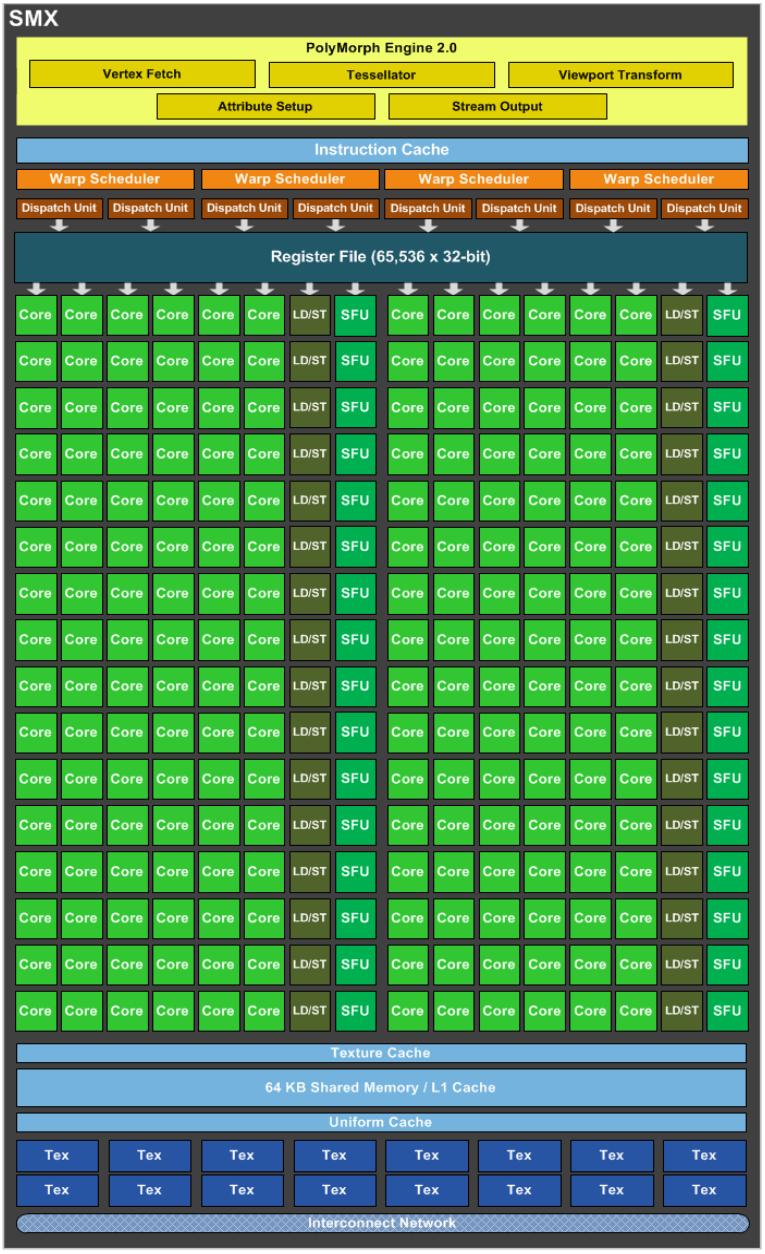
\includegraphics[width=0.8\textwidth]{SMX}
	\end{center}
	\caption{GK-104 Streaming Multiprocessor (SMX) block diagram \cite{GK-104 Whitepaper}.}
	\label{fig:SMX}
\end{figure}

\begin{table}[tb]
	\caption{GK-104 functional units per SMX \cite{Anand}.}
	\label{tab:funcunits}
	\begin{center}
		\begin{tabular}{rl}
		\hline

		\hline
		\textbf{width} & \textbf{Type} \\
		\hline
			32 & CUDA cores (\#1) \\
			32 & CUDA cores (\#2) \\
			32 & CUDA cores (\#3) \\
			32 & CUDA cores (\#4) \\
			32 & CUDA cores (\#5) \\
			32 & CUDA cores (\#6) \\
			16 & Load/Store Units (\#1) \\
			16 & Load/Store Units (\#2) \\
			16 & Interpolation SFUs (\#1) \\
			16 & Interpolation SFUs (\#2) \\
			16 & Special Function SFUs (\#1) \\
			16 & Special Function SFUs (\#2) \\
			8 & Texture Units (\#1) \\
			8 & Texture Units (\#2) \\
			8 & CUDA FP64 cores \\
		\hline

		\hline
		\end{tabular}
	\end{center}
\end{table}

% subsection introduction_to_the_gk_104 (end)

\subsection{Initial GPU implementation} % (fold)
\label{sub:initial_implementation}
The starting point for the GPU version was a straightforward CUDA rewrite of kernels as follows:

As discussed above, the default boundary condition setting \texttt{expression 1} kernel was inefficiently iterating over cells to initalise the node array, overwriting adjacent cells' results and therefore doing a factor of roughly 36 redundant work for the given small mesh. The CUDA kernel version iterates directly over the array (each iteration packed into a separate thread). It is worth noting that the boundary code uses cosines, which are accelerated in hardware on the GPU and thus are significantly faster.

The \texttt{zero} kernel was turned into a cudaMemset, executing in a millisecond.

The \texttt{expression 2} kernel was observed to be doing a trivial direct copy operation, which is removed by simply passing the original buffer pointer to the next kernel.

For \texttt{rhs} and \texttt{lhs} kernels, each thread performs the whole computation over a cell (i.e. the 8x6x6 nested loop). The threads are packed into blocks in column order, to allow adjacent threads in a warp to do coalesced reads and writes to input/output data as it is stored sequentially for a column of nodes. As in the TBB version, accumulation of results to the global vector was made atomic.

To verify correctness, buffer states after each kernel pass were copied to the host and compared against the results of its reference computation. Naturally, for release builds, all memory is kept on the device until the final output buffer copy back.

% subsection initial_implementation (end)

\subsection{Constant Memory Optimisation} % (fold)
\label{sub:constant_memory_optimisation}

\begin{figure}[tb]
	\begin{center}
		\includegraphics[width=\textwidth]{"Original nonconst LHS memory overview BW"}
	\end{center}
	\caption{Memory bandwidth overview of original implementation}
	\label{fig:membBWorig}
\end{figure}

\begin{figure}[tb]
	\begin{center}
		\includegraphics[width=\textwidth]{"LHS memory overview BW"}
	\end{center}
	\caption{Memory bandwidth overview of constant memory implementation}
	\label{fig:membBWfinal}
\end{figure}

Profiling the initial imoplementation we see that the memory bandwith to local memory is very high, and that the L1 and L2 cache hits are very low, and therefore we have a lot of local memory transactions to off-chip memory. This is shown in Figure~\ref{fig:membBWorig}.
Checking the disassembly, we see that the large constant matricies used in the computation is pushed onto the stack, which is stored in local memory.
Even though these matricies are constant across all threads in the kernel, they each have a destinct stack, and therefore the L1 and L2 cache will not properly cache the access to these matricies.
Therefore, as these matricies are then accessed in the hot loop of the kernels, prompts several fetches from off-chip memory for every iteration. This makes for very poor performance.

The GK-104 offeres a special constant-memory cache which is destinct from the L1 and L2 cache. This cache will only store variables which are declared in global scope and with the \verb.__constant__. qualifier.

\begin{table}[tb]
	\caption{Comparison of execution times for constant memory optimisation on small mesh.}
	\label{tab:constMemExeTime}
	\begin{center}
		\begin{tabular}{l|cc|cc}
		\hline

		\hline

		& \multicolumn{2}{c|}{\textbf{Execution time}} & \multicolumn{2}{c}{\textbf{Local Memory Use}} \\
		\textbf{Memory} & \textbf{Local} & \textbf{Constant} & \textbf{Local} & \textbf{Constant} \\
		\hline
			\textbf{Kernel} &&&&\\
			LHS 	& 3.08 	& 1.28 & 385GB & 93GB \\
			All 	& 5.68 	& 2.58 \\
		\hline

		\hline
		\end{tabular}
	\end{center}
\end{table}

% subsection constant_memory_optimisation (end)

\subsection{Reducing register spill} % (fold)
\label{sub:reducing_register_spill}

\begin{itemize}
	\item Transpose attempt
	\item Fail : ILP? IP-k result reuse?
	\item Final version: 2x6 accum streams, for: ip, k, j (2k 6j streams)
\end{itemize}

\begin{lstlisting}[frame=, language=C++, caption=LHS kernel main loop]
for (int ip = 0; ip<8; ip++){
	for (int k = 0; k<6; k++){
		for (int j = 0; j<6; j++){
			A[k%2][j] += LargeExpression;
		}
	}
}
\end{lstlisting}

% subsection reducing_register_spill (end)

\subsection{Final Profiling} % (fold)
\label{sub:final_profiling}

\begin{figure}[tb]
	\begin{center}
		\includegraphics[width=\textwidth]{"LHS efficency and stall reason"}
	\end{center}
	\caption{LHS issue efficency and stall reasons}
	\label{fig:issue_eff_and_stall_reasons}
\end{figure}

\begin{itemize}
	\item DP Structural Hazard ultimate bottleneck
\end{itemize}

This suggests that if double precision is nessecary for the application, then perhaps the GK-104 is not the best choice. Indeed, the GK-110 has 64 double precision units per SMX, and would be a much better choice for this workload.

As a consequence, a small benefit is that the thermal output of the device is less than 75\% of TDP. This means that the Dynamic Voltage and Freqency Scaling (DVFS) system will clock the GPU at its maximum frequency all the time.

% subsection final_profiling (end)


% section gpu_and_cuda (end)

\section{Work partition} % (fold)
\label{sec:work_partition}
\begin{tabular}{ l l  }
Yong Wen Chua & - TBB, CUDA. \\
Oskar Weigl & - CUDA, profiling. \\
Ryan Savitski & - code analysis. \\
\end{tabular}
% section work_partition (end)

\clearpage
\begin{appendices}
\section{Summary and setup}

\subsection{CPU} % (fold)
\label{sub:cpu}

\begin{verbatim}
Processor 1     ID = 0
  Number of cores   4 (max 8)
  Number of threads 8 (max 16)
  Name      Intel Core i7 3770K
  Codename    Ivy Bridge
  Specification   Intel(R) Core(TM) i7-3770K CPU @ 3.50GHz
  Package (platform ID) Socket 1155 LGA (0x1)
  CPUID     6.A.9
  Extended CPUID    6.3A
  Core Stepping   E1/L1
  Technology    22 nm
  TDP Limit   77 Watts
  Tjmax     105.0 °C
  Core Speed    2807.4 MHz
  Multiplier x Bus Speed  28.0 x 100.3 MHz
  Stock frequency   3500 MHz
  Instructions sets MMX, SSE, SSE2, SSE3, SSSE3, SSE4.1, SSE4.2, EM64T, VT-x, AES, AVX
  L1 Data cache   4 x 32 KBytes, 8-way set associative, 64-byte line size
  L1 Instruction cache  4 x 32 KBytes, 8-way set associative, 64-byte line size
  L2 cache    4 x 256 KBytes, 8-way set associative, 64-byte line size
  L3 cache    8 MBytes, 16-way set associative, 64-byte line size
  FID/VID Control   yes

  Turbo Mode    supported, enabled
  Max non-turbo ratio 35x
  Max turbo ratio   39x
  Max efficiency ratio  16x
  Min Power   60 Watts
  O/C bins    unlimited
  Ratio 1 core    39x
  Ratio 2 cores   39x
  Ratio 3 cores   38x
  Ratio 4 cores   37x
  TSC       3510.2 MHz
  APERF     3730.9 MHz
  MPERF     3481.3 MHz
\end{verbatim}

\clearpage

\subsection{GPU} % (fold)
\label{sub:gpu}
\begin{verbatim}
Display adapter 0 
  Name      NVIDIA GeForce GTX 670
  Revision    A2
  Codename    GK104
  Technology    28 nm
  Memory size   2 GB
  PCI device    bus 1 (0x1), device 0 (0x0), function 0 (0x0)
  Vendor ID   0x10DE (0x3842)
  Model ID    0x1189 (0x2678)
  Performance Level 0
    Core clock  1175.0 MHz
    Memory clock  3105.0 MHz

Win32_VideoController   AdapterRAM = 0x80000000 (2147483648)
Win32_VideoController   DriverVersion = 9.18.13.3523
Win32_VideoController   DriverDate = 03/04/2014
\end{verbatim}

\subsection{Operating system} % (fold)
\label{sub:operating_system}
\begin{verbatim}
Windows Version     Microsoft Windows 7 (6.1)
                    Ultimate Edition 64-bit  Service Pack 1 (Build 7601) 
\end{verbatim}

\subsection{Parallelisation paradigms} % (fold)
\label{sub:parallelisation_paradigms}
Intel Threading Building Blocks on the host CPU during initial investigations. CUDA on GPU.
% subsection parallelisation_paradigms (end)

\subsection{CUDA} % (fold)
\label{sub:cuda}
Compiler:
\begin{verbatim}
nvcc: NVIDIA (R) Cuda compiler driver
Built on Wed_Jul_10_13:36:45_PDT_2013
Cuda compilation tools, release 5.5, V5.5.0
\end{verbatim}
Compilation flags:
\begin{verbatim}
nvcc.exe -gencode=arch=compute_30,code=\"sm_30,compute_30\" --use-local-env 
         --cl-version 2012 -maxrregcount=0  --machine 64 --compile -cudart static 
         -DWIN64 -DNDEBUG -D_CONSOLE -D_MBCS -Xcompiler "/EHsc /W3 /nologo /O2 /Zi /MD"
\end{verbatim}



\end{appendices}
%%%%%%%%%%%%%%%%%%%%%%%%%%%%%%%%%%%%%%%%%%%%%%%%%%%%%%%%%%%%%%%%%%%%%%%%%%%%%%%%%%%%%%%%%%%%%%%%%%%%%%%%%%%%%%%%%%%%%
%%%%%%%%%%%%%%%%%%%%%%%%%%%%%%%%%%%%%%%%%%%%%%%%%%%%%%%%%%%%%%%%%%%%%%%%%%%%%%%%%%%%%%%%%%%%%%%%%%%%%%%%%%%%%%%%%%%%%
%%%%%%%%%%%%%%%%%%%%%%%%%%%%%%%%%%%%%%%%%%%%%%%%%%%%%%%%%%%%%%%%%%%%%%%%%%%%%%%%%%%%%%%%%%%%%%%%%%%%%%%%%%%%%%%%%%%%%
%%%%%%%%%%%%%%%%%%%%%%%%%%%%%%%%%%%%%%%%%%%%%%%%%%%%%%%%%%%%%%%%%%%%%%%%%%%%%%%%%%%%%%%%%%%%%%%%%%%%%%%%%%%%%%%%%%%%%


\hspace{1em}
\hrule
general notes
\hspace{1em}
\hrule

\section{report notes \& deliverables} % (fold)
\label{sec:report_notes_on_deliverables}

Marks are awarded for:
\begin{itemize}
\item  Systematic analysis of the application's behaviour
\item  Systematic evaluation of performance improvement hypotheses
\item  Drawing conclusions from your experience
\item  A professional, well-presented report detailing the results of your work.
\end{itemize}

\subsection{} % (fold)
\label{sub:}

% subsection  (end)

What to hand in Hand in a concise report which
\begin{itemize}
\item  Explains what hardware and software you used,
\item  What hypothesis (or hypotheses) you investigated,
\item  How you evaluated what the potential advantage could be,
\item  How you explored the effectiveness of the approach experimentally
\item  What conclusions can you draw from your work
\item  Specify how you ensured the correct results were obtained or justify why that is not the case
\item  If you worked in a group, indicate who was responsible for what.
\end{itemize}

\subsection{} % (fold)
\label{sub:}

% subsection  (end)

Regarding the report for the Helmholtz challenge, to make marking easier in terms of the technical side of your experiments, and also to gain a clear understanding of what you did/tried I would like you to include a structured summary of the outcome of the various optimizations attempted.

Ideally this would be a table specifying:
\begin{itemize}
\item  the hardware you ran on including: CPU/GPU, processor model number, clock rate, number of cores, cache sizes
\item  the compiler you used: ICC, GCC, etc, the compiler version number
\item  the compiler flags -fopenmp -Ofast -avx  - or whatever your choice is
\item  the parallelization strategy/paradigm used, if any (threads, OpenMP,OpenCL, MPI, CUDA)
\item  the number or range of cores you ran on
\item  the execution times you measured, and the steps you took to ensure your results are reproducible (ie not subject to random variations)
\item  the speed-up you got. If it helps you can point to graphs in your report.
\end{itemize}
If you have tried several improvements to the code or you would like to show how you explored a certain range of optimizations then you can include intermediate results which show the effect of a particular optimization.

This table needn't be longer than half a page (a page at most if you really really have to) and should make the presentation of the results concise.  This can be outside your page budget.

% section report_notes_on_deliverables (end)

\clearpage

%INstruction throughput table
%http://docs.nvidia.com/cuda/cuda-c-programming-guide/index.html#arithmetic-instructions__throughput-native-arithmetic-instructions

%GK 104 Whitepaper
%http://www.geforce.com/Active/en_US/en_US/pdf/GeForce-GTX-680-Whitepaper-FINAL.pdf

%Anandtech article (functional units division)
%http://www.anandtech.com/show/5699/nvidia-geforce-gtx-680-review/2

\begin{thebibliography}{9}

  \bibitem{tbbr}
  Intel,
  \emph{Intel Threding Building Blocks}. \\
  \url{https://www.threadingbuildingblocks.org}

  \bibitem{QPC}
  Microsoft,
  \emph{Developer reference - QueryPerformanceCounter function}. \\
  \url{http://msdn.microsoft.com/en-us/library/windows/desktop/ms644904(v=vs.85).aspx}

	\bibitem{GK-104 Whitepaper}
	Nvidia,
	\emph{Whitepaper - NVIDIA GeForce GTX 680}. \\
	\url{http://www.geforce.com/Active/en_US/en_US/pdf/GeForce-GTX-680-Whitepaper-FINAL.pdf}

	\bibitem{Anand}
	Ryan Smith,
	\emph{The Kepler Architecture: Fermi Distilled}. \\
	\url{http://www.anandtech.com/show/5699/nvidia-geforce-gtx-680-review/2}

	\bibitem{Progguide Instruction throughput}
	Nvidia,
	\emph{Cuda-C Programming Guide - Table 2. Throughput of Native Arithmetic Instructions}. \\
	\url{http://docs.nvidia.com/cuda/cuda-c-programming-guide/index.html#arithmetic-instructions__throughput-native-arithmetic-instructions}

\end{thebibliography}

\end{document}


%%%%%%%%%%%%%%%%%%%%%%%%%%%%%%%%%%%%%%%%%%%%%%%%%%%%%%%%%%%%%%%%%%%%%%%%%%%%%%%%%%%%%%%%%%%%%%%%%%%%%%%%%%%%%%%%%%%%%
%%%%%%%%%%%%%%%%%%%%%%%%%%%%%%%%%%%%%%%%%%%%%%%%%%%%%%%%%%%%%%%%%%%%%%%%%%%%%%%%%%%%%%%%%%%%%%%%%%%%%%%%%%%%%%%%%%%%%
%%%%%%%%%%%%%%%%%%%%%%%%%%%%%%%%%%%%%%%%%%%%%%%%%%%%%%%%%%%%%%%%%%%%%%%%%%%%%%%%%%%%%%%%%%%%%%%%%%%%%%%%%%%%%%%%%%%%%
%%%%%%%%%%%%%%%%%%%%%%%%%%%%%%%%%%%%%%%%%%%%%%%%%%%%%%%%%%%%%%%%%%%%%%%%%%%%%%%%%%%%%%%%%%%%%%%%%%%%%%%%%%%%%%%%%%%%%
data parallel
tons of independent work
fp calculations


accel of cos-field through hw

const mem


register spilling in base cuda implementation
%%%%%%%%%%%%%%%%%%%%%%%%%%%%%%%%%%%%%%%%%%%%%%%%%%%%%%%%%%%%%%%%%%%%%%%%%%%%%%%%%%%%%%%%%%%%%%%%%%%%%%%%%%%%%%%%%%%%%
%%%%%%%%%%%%%%%%%%%%%%%%%%%%%%%%%%%%%%%%%%%%%%%%%%%%%%%%%%%%%%%%%%%%%%%%%%%%%%%%%%%%%%%%%%%%%%%%%%%%%%%%%%%%%%%%%%%%%
so: to write about in report (if you want to still focus on that): interchange does free up registers, reduces register spilling to the point of 0 if you do both i and j outside. However, most likely the compiler is hiding the serial latency of the massive serial sum of products statement using the iterations over i and j.
therefore, returning to the same accumulator quickly, you lose performance


[21:29:03] madcowswe: what is really interesting to write about is the ability for the compiler to do interleaving of different iterations to hide the latency (:
%%%%%%%%%%%%%%%%%%%%%%%%%%%%%%%%%%%%%%%%%%%%%%%%%%%%%%%%%%%%%%%%%%%%%%%%%%%%%%%%%%%%%%%%%%%%%%%%%%%%%%%%%%%%%%%%%%%%%
%%%%%%%%%%%%%%%%%%%%%%%%%%%%%%%%%%%%%%%%%%%%%%%%%%%%%%%%%%%%%%%%%%%%%%%%%%%%%%%%%%%%%%%%%%%%%%%%%%%%%%%%%%%%%%%%%%%%%
%%%%%%%%%%%%%%%%%%%%%%%%%%%%%%%%%%%%%%%%%%%%%%%%%%%%%%%%%%%%%%%%%%%%%%%%%%%%%%%%%%%%%%%%%%%%%%%%%%%%%%%%%%%%%%%%%%%%%


\section{General Approach}

The general approach taken to speed up the execution of the calculation is to exploit the parallelism inherent in the problem itself. In particular, by studying the source code, we can see that for each of the wrapper function calls, the cells calculations are mostly independent of each other. The cell calculations can therefore be made to run in parallel. Due to unstructured nature of the mesh, calculations over the entire space must be complete before the next call to the next wrapper function can be made.

In each of the cell, calculation is written to a buffer in which each element of the buffer corresponds to one vertex in the mesh. Since a vertex can belong to more than one cell, care must be taken to ensure that the values accumulated in each vertex is done so without any race conditions such as an atomic add.

The unstructured nature of the mesh also means that trying to exploit spatial locality might be difficult. It will also be difficult to divide the entire iteration space into independent blocks because the memory locations are not ``adjacent'' to each other. 

\section{Threading}

The first approach to speeding up the calculation was to use threads to exploit the parallelism inherent in the problem. Using the Threading Building Blocks library\footnote{https://www.threadingbuildingblocks.org/}, the iteration space was made into what is essentially a parallel for loop that the library can schedule to run in parallel using threads depending on the hardware available. 

There are two avenues for parallerise the work being done: over each ``column'' of cells or over each cell individually.  We hypothesise that while both variants of threading will bring about performance improvements to the computation over the original serialised version, the former parallel version is expected to work better than the latter. This is because the work done per cell might be too small compared to the overheads of thread scheduling and context switching. 

The results shown in table \ref{table:threads} confirms our hypothesis. We notice that threading by columns gives the largest amount of speed up over the original version, by approximately a factor of four. For threading by cell, the performance for most operations are improved significantly, though not as much as threading by columns. Finally, interpolating expressions became slower in this version because of the overheads in thread scheduling when each thread does too little work.

\section{CUDA Acceleration}




\section{Summary Table}
\subsection{Threading Performance}
Testing was done on a laptop with Intel Core i7-4700MQ with 4 cores running on Linux 13.10. The programs were compiled with GCC with optimisation set to level 3. The results are summarised in the table below, and the times are consistent across several runs with very minor variations. The times for the steps ``Set array to zero'' and ``Evaluating expression'' are not reported because they are trivial cases that has been optimised by the compiler. The timings were generated from the large mesh.

\begin{table}[h]
\begin{tabularx}{1.2\textwidth}{ |X|X|X|X|X| }
\cline{2-5}
                                          & Evaluating Exp & Interpolating Exp & Assembling RHS & Assembling LHS \\ \hline
\multicolumn{1}{|l|}{Original Version}    & 40.0307        & 4.86542           & 21.0748        & 37.747         \\ \hline
\multicolumn{1}{|l|}{Threading by Cell}   & 12.993         & 5.59316           & 11.0813        & 14.9041        \\ \hline
\multicolumn{1}{|l|}{Threading by Column} & 7.77536        & 1.19127           & 5.64956        & 9.59484        \\ \hline
\end{tabularx}

\caption{Timings in seconds for threaded version using the large data mesh.}
\label{table:threads}
\end{table}
\subsection{CUDA Performance}

\end{document}
